
\chapter{Machine Learning}

From Netflix recommendations to self-driving cars, to the stock market, machine learning (ML) is quietly shaping the
systems we use every day. But what is it, really?

At its heart, machine learning is about teaching computers to learn from experience. In a standard setting, this is like teaching a
child to recognize a cat by showing them lots of pictures and giving feedback. Instead of writing a long, rigid list of rules (like
``if it has pointy ears and whiskers, it's a cat''), we let the computer discover the patterns in the data and improve its own
performance over time.

Today, ML powers everything from voice assistants to medical diagnosis. In finance, it helps spot fraud, optimize portfolios, and
predict future market direction. But financial machine learning has a unique challenge: unlike a clear picture of a cat, market data
is incredibly noisy.

That is why the secret to algorithmic trading isn't just building a complex model; it's getting the data right to begin with. As you saw in the last chapter, high-quality, stationary data that preserves market memory is the real fuel for
any financial ML system.

In this chapter, we'll focus on the most practical and widely used branch for our pipeline: supervised learning. We'll also briefly
introduce unsupervised and reinforcement learning, so you see the big picture. You'll learn what makes each approach unique, how
algorithms use "decision trees" to mimic human logic, and how they fit into the system you've already started building. By the end,
you'll be ready to judge whether your model is actually uncovering a true market signal, or just memorizing historical flukes.

\section{Principles of Machine Learning}

Before we dive into the mechanics of machine learning, let us pause and consider how algorithms already shape our daily lives.
Every time you unlock your phone with your face, get a movie suggestion from Netflix, or follow a recipe to bake cookies, you are relying on algorithms at work.
These are not just abstract computer concepts, they are the invisible instructions guiding everything from your morning routine to the apps you use.
In fact, we have all been using algorithms our entire lives, often without realizing it. Whether you are tying your shoes, solving a Rubik's cube, or deciding what to eat for breakfast, your daily routines are full of these stepwise procedures.
So, what exactly is an \textbf{algorithm}? Think of it as a recipe: a clear, step-by-step set of instructions for turning raw ingredients (your input) into a finished dish (your output).
In machine learning, algorithms are the backbone: they tell the computer exactly how to turn real-world data into useful predictions or decisions. 

In traditional programming, a developer writes explicit rules that the computer must follow, a series of \texttt{if-then-else} statements and conditions that form the basis of a program.
Want to detect spam email? A traditional programmer might write: ``\textit{if the subject line contains the word `FREE' and the sender is unknown, mark as spam.}''
This works reasonably well,  until the spammers start writing ``FR\$\$'' instead of ``FREE,'' and the programmer has to update the rules again.
The fundamental limitation is clear: \textit{the programmer must anticipate every case in advance}. 

\textbf{Machine learning} (ML) flips this model on its head. Rather than a human writing the rules, we give the computer \textit{examples} of correct behavior and let the computer \textit{figure out the rules itself}.
Feed it thousands of spam emails and thousands of legitimate ones, and the algorithm will discover, on its own, what patterns distinguish the two!  
This shift, from rule-writing to example-showing, is the core idea that makes machine learning so powerful and so different from everything that came before it (see Figure~\ref{fig:traditional_vs_ml}). 
In traditional programming, data and rules go \textit{in}, and answers come \textit{out}. 
In machine learning, data and answers (examples) go \textit{in}, and \textit{rules} come out. 
The output of a machine learning system is not a prediction by itself. In this context, a model is a compact, learned representation of the patterns in the data that can then be applied to new, unseen inputs.

Given how central machine learning has become, it's natural to wonder: if the field has existed since the 1950s, why are we only now seeing it become so widespread?
The practical answer lies in two major limitations that held the field back for decades: the availability of large, high-quality datasets, and the sheer amount of computing power required. Machine learning is, at its core, a way to overcome a lack of explicit knowledge by leveraging an abundance of data. For much of its history, this abundance simply did not exist. The advent of cloud computing and advances in computer technology have enabled researchers and companies not only to store and process vast amounts of data, but also to access it seamlessly from anywhere in the world over the internet. Seemingly, companies across the world had a collective awakening to the importance of data collection and information modeling. This shift was not just about better algorithms, but about the sudden availability of massive datasets and the computing power, especially GPUs, needed to process them \cite{ibm2012bigdata,idc2021datasphere}.
To put this explosion in perspective: in 2010, the world generated about 2 zettabytes of data over the entire year. \cite{statista2024data,idc2021datasphere}. 
Today, we generate roughly 402 million terabytes of data every single day \cite{statista2024data}. For scale, one zettabyte is equal to one billion terabytes \cite{nistZB}. 
Data collection has become so desirable that companies are even offering hardware products for free, simply to gather consumer usage data. This relentless pursuit of information underscores how valuable data has become in the modern economy, fueling advances in machine learning and finance alike.

For decades, computing was all about the Central Processing Unit (CPU). 
The CPU was the ``chef'' in the kitchen, following recipes (programs) step by step, one dish at a time.
Programs were written, compiled or interpreted, and executed via the CPU, which excelled at handling a wide variety of tasks, but only a few at once.
Incremental improvements in CPU performance have mostly come from smarter designs—such as adding more cores (moving from single-core to quad-core and beyond), refining how instructions are processed, and squeezing out more parallelism where possible. 
But even with these advances, CPUs are still generalists: great at juggling many different tasks, but not built for the kind of massive, simultaneous number-crunching that modern machine learning demands.
Researchers 

For the last twenty years, it was widely claimed by the media, politicians, and parents, that the video game industry wouldn't amount to much.
Ironic, isn't it? The same industry, once dismissed as a frivolous pastime, became the unlikely hero in the story of machine learning's rise. 
Why? Because the relentless quest for ever more realistic graphics, such as lifelike shadows, explosions, and shimmering water, drove the development of the Graphical Processing Unit (GPU).
Rendering a single video game scene means calculating the color and brightness of millions of pixels, all at once. 
Each calculation is simple, but there are so many of them that only a processor designed for massive parallelism can keep up.
This native design, centered around parallel processing, is perfectly suited for machine learning. 
Training a modern ML model rarely requires solving one giant, complicated equation. 
Instead, it involves doing millions of simple math operations, like matrix multiplications, at the same time.
If a CPU is like one brilliant professor, a GPU is a stadium filled with 10,000 diligent students. Individually, each student can only do basic arithmetic, but working together, they can crunch through mountains of data.

When researchers realized they could repurpose gaming GPUs to train machine learning models, the field exploded. 
Algorithms that used to take months to train on a traditional computer could suddenly be completed in a few hours.
Today, with the rise of cloud computing, this barrier has been significantly lowered. 
You no longer need to buy a supercomputer to run advanced financial models. 

This democratization of cheap, powerful computation has opened the door for financial machine learning, allowing even small teams to build and test sophisticated trading algorithms that once required the resources of Wall Street giants.


% Requires: tcolorbox, tikz, xcolor (with darkred, darkgreen defined in preamble)

\begin{figure}[ht]
\centering
\begin{tikzpicture}[
    box/.style={draw, rounded corners=3pt, minimum width=3.8cm, minimum height=1.2cm, align=center, font=\small},
    arrow/.style={->, thick, >=stealth},
    label/.style={font=\footnotesize\itshape, text width=2.5cm, align=center}
]

% ============ TRADITIONAL PROGRAMMING (Left) ============
\node[font=\bfseries\sffamily, text=darkred] at (-4.5, 3.2) {Traditional Programming};

% Input boxes
\node[box, fill=gray!10] (data1) at (-5.8, 1.8) {Data};
\node[box, fill=red!10, draw=darkred] (rules1) at (-3.2, 1.8) {Rules\\{\footnotesize (written by you)}};

% Computer box
\node[box, fill=blue!8, draw=blue!40!black, minimum width=4cm] (computer1) at (-4.5, 0) {Computer};

% Output box
\node[box, fill=green!10, draw=darkgreen] (output1) at (-4.5, -1.8) {Answers};

% Arrows
\draw[arrow] (data1.south) -- ++(0,-0.4) -| (computer1.north west);
\draw[arrow] (rules1.south) -- ++(0,-0.4) -| (computer1.north east);
\draw[arrow] (computer1.south) -- (output1.north);

% Labels
\node[label, anchor=east] at (-6.8, 1.8) {input};
\node[label, anchor=west] at (-2.2, 1.8) {input};
\node[label, anchor=east] at (-6.2, -1.8) {output};

% ============ DIVIDER ============
\draw[thick, dashed, gray] (0, 3.5) -- (0, -2.8);
\node[font=\Large\bfseries, gray] at (0, -3.2) {vs};

% ============ MACHINE LEARNING (Right) ============
\node[font=\bfseries\sffamily, text=darkgreen] at (4.5, 3.2) {Machine Learning};

% Input boxes
\node[box, fill=gray!10] (data2) at (3.2, 1.8) {Data};
\node[box, fill=green!10, draw=darkgreen] (answers2) at (5.8, 1.8) {Answers\\{\footnotesize (examples)}};

% Computer box
\node[box, fill=blue!8, draw=blue!40!black, minimum width=4cm] (computer2) at (4.5, 0) {Computer};

% Output box
\node[box, fill=red!10, draw=darkred] (rules2) at (4.5, -1.8) {Rules\\{\footnotesize (learned model)}};

% Arrows
\draw[arrow] (data2.south) -- ++(0,-0.4) -| (computer2.north west);
\draw[arrow] (answers2.south) -- ++(0,-0.4) -| (computer2.north east);
\draw[arrow] (computer2.south) -- (rules2.north);

% Labels
\node[label, anchor=east] at (2.2, 1.8) {input};
\node[label, anchor=west] at (6.8, 1.8) {input};
\node[label, anchor=west] at (6.2, -1.8) {output};

\end{tikzpicture}

\vspace{1em}

\begin{tcolorbox}[
    colback=blue!3!white,
    colframe=blue!40!black,
    arc=2pt,
    boxrule=0.5pt,
    width=0.95\textwidth,
    halign=center,
    top=3pt, bottom=3pt
]
\textbf{Key insight:} In traditional programming, \emph{you} write the rules. In machine learning, the algorithm \emph{discovers} the rules by studying examples.
\end{tcolorbox}

\caption{Traditional programming versus machine learning. On the left, the programmer supplies both data and hand-coded rules; the computer produces answers. On the right, the programmer supplies data and example answers; the computer produces the rules (a trained model).}
\label{fig:traditional_vs_ml}
\end{figure}


\section{Supervised Learning}

Historically, epigraphy (the study of ancient inscriptions) was a painstakingly manual process, requiring years of linguistic expertise and comparison with known texts like the Rosetta Stone.
The process involved meticulous analysis of symbols, their contexts, and their relationships to one another.
Researchers would document each symbol, cross-reference it with known languages, and gradually piece together the meanings.
In 2017, Ubisoft, a video game company, launched a research project called \textit{The Hieroglyphics Initiative} to coincide with the release of their game Assassin's Creed Origins (which is set in ancient Egypt).
Their goal was to see if machine learning could streamline the cataloging of the pharaohs' language.
They did this by training a machine learning model on a large set of examples, like a stack of flashcards with both the hieroglyph and its translation.
While it took centuries for scholars to build the catalog of known Egyptian symbols, a supervised model can process thousands of images in seconds, flagging uncertain symbols for human review and drastically reducing the manual labor of epigraphy.
The model performed remarkably well, accurately identifying the majority of hieroglyphs and demonstrating that AI could significantly accelerate the study and translation of ancient texts while still relying on human expertise for ambiguous cases.

This application of machine learning is known as \textbf{supervised learning}, where the model is trained on a labeled dataset, learning to map inputs (like images of hieroglyphs) to outputs (their translations). 
This pattern, learning from examples with known answers, underpins everything from image recognition to predicting tomorrow's stock price.

Supervised learning is a type of machine learning where the model is trained on a \textbf{labeled dataset}, meaning that each input data point is paired with the correct output. 
The model learns to map inputs to outputs by finding patterns in the data. Once trained, the model can make predictions on new, unseen data. 
This labeled dataset is broken into two key pairs: \textbf{features} and \textbf{labels}. 
Features are the measurable properties or characteristics of the data, while labels are the outcomes or targets that we want to predict.

In our financial context, features might include recent price changes, trading volume, or technical indicators such as the relative strength index or exponential moving average. Labels are the outcomes we want to predict—like whether a trade will be profitable or not.

For many years, researchers tried to predict the exact next price of an asset. 
But as we've discussed in previous chapters, so many unpredictable factors influence price that this is a daunting task. Instead, we often simplify the problem: rather than guessing the next price, we ask the model to classify the next movement as ``profitable'' or ``unprofitable'' for a given trading strategy.

This leads to two main types of supervised learning problems:
\begin{itemize}
	\item \textbf{Classification:} The model assigns each input to a category, such as ``profitable'' or ``unprofitable.'' For example, using a moving average crossover strategy, the model learns from historical data to predict whether the next trade will succeed or not.
	\item \textbf{Regression:} The model predicts a continuous value, like the exact next price of an asset.
\end{itemize}

In this book, we'll focus mainly on classification, since it's often more practical and robust in financial applications.
In traditional programming, we know a developer is responsible for the rules, but we noted that ML flips this model on its head. 
So, how does a model actually learn from the data?
If anyone remembers a game called ```20 Questions''' you can relate to how a model learns. 
In this game, one player thinks of an object, and the other player asks yes/no questions to narrow down the possibilities.
In a similar way, a machine learning model learns by asking questions about the features in the data. 
Similar to the different strategies a player might use in 20 Questions, there are different algorithms that can be used to learn from a dataset, each with its own strengths and weaknesses.

\begin{itemize}
    \item \textbf{transformers/CNN} transformers and convolutional neural networks (CNNs) are powerful for processing sequential or spatial data, such as time series or images.
    \item \textbf{decision trees} decision trees are a simple yet effective algorithm that splits the data into branches based on feature values, making decisions at each node.
    \item \textbf{random forests} random forests are an ensemble method that combines multiple decision trees to improve accuracy and reduce overfitting.
    \item \textbf{gradient boosting} gradient boosting is another ensemble technique that builds trees sequentially, where each new tree corrects the errors of the previous ones.
\end{itemize}

In the next section, we'll explore how decision trees work, and why they are a popular choice for financial machine learning applications. 
We'll also discuss how to evaluate the performance of these models and ensure they generalize well to new data, rather than just memorizing historical patterns.

\section{Random Forest}


Have you ever played 20 Questions with a friend? If so, you've already used a decision tree!

In our previous section, we introduced multiple supervised learning algorithms, including decision trees and ensemble methods like random forests. A decision tree is just a hierarchical structure (top-down) that splits the data into branches based on feature values, making decisions at each node. A model reaches a decision by traversing a decision tree from the \textbf{root node} to a \textbf{leaf node}, where the final prediction is made.

The root node is the topmost node in a decision tree, representing the entire dataset. A leaf node, on the other hand, is a terminal node that provides the final output or prediction for a given input. It's a node without any child nodes (branches), and it represents the end of a decision path in the tree.

Along the way, the model passes through internal nodes. Think of these as the decision points where you ask, ``Does it live in water?'' or ``Is it man-made?''

In the example visualized in Figure~\ref{20q}, a 5-level decision tree is used to play the game of 20 Questions. The root node in this case is \textit{Is it a living thing?}. There are several internal nodes such as \textit{Does it live in water?}, \textit{Is it an animal?}, and \textit{Is it man-made?}. The leaf nodes represent the final answers, such as \textit{whale}, \textit{tree}, or \textit{rock}.

\begin{figure}[ht]
  \centering
  \label{20q}
  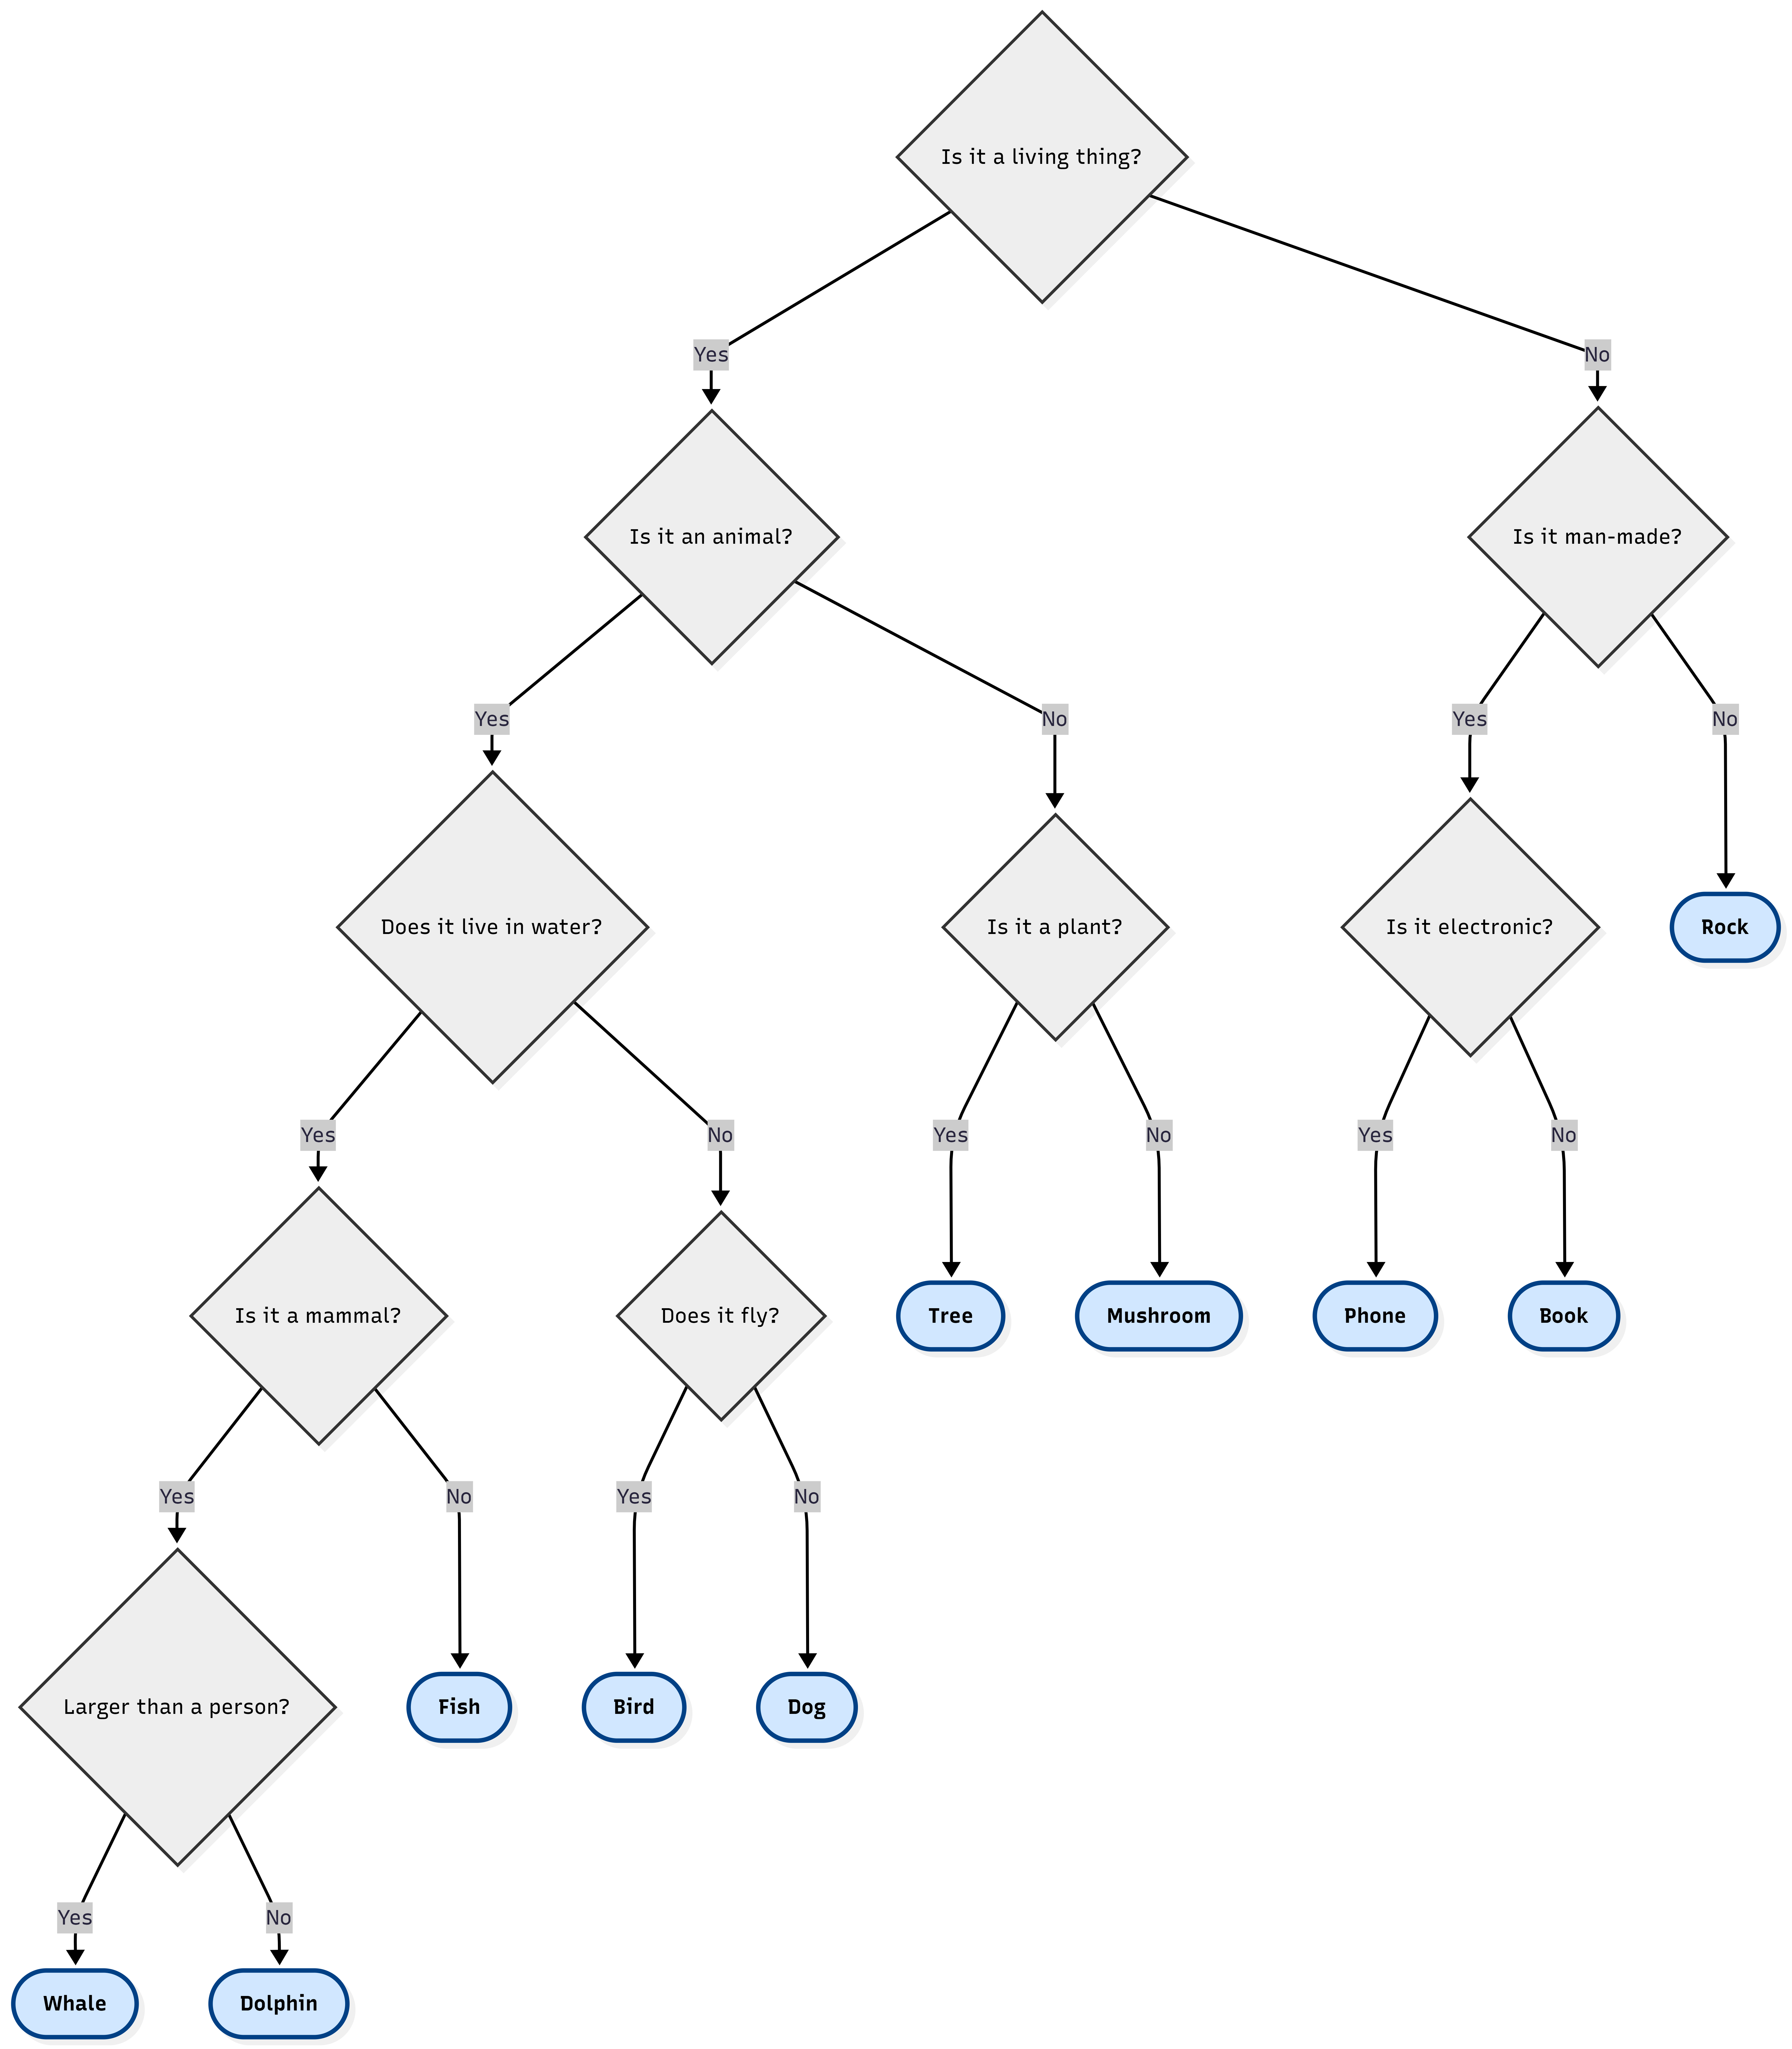
\includegraphics[width=0.8\textwidth]{figures/chapter0x/DecisionTreeClassification.png}
  \caption{A 5-level decision tree for 20 Questions.}
\end{figure}